\section{Kernelspace variant based on dynamic instrumentation}
\label{appfw:appscout}

%%%%%%%%%%%%%%%%%%%%%%%%%%%%%%%%%%%%%%%%%%%%%%%%%%%%%%%%%%%%%%%%%%%%%%%%%%%%%%%%
\subsection{Problem statement}

\radu{TODO: introduce AppScout}

%%%%%%%%%%%%%%%%%%%%%%%%%%%%%%%%%%%%%%%%%%%%%%%%%%%%%%%%%%%%%%%%%%%%%%%%%%%%%%%%
\subsection{Architecture}
\label{apffw:appscout:architecture}

In this subsection we describe the architecture of \scout{}. Figure
\ref{appfw:appscout:fig:sys-architecture} offers a high-level overview of the
modules that comprise our firewalling solution (i.e., the primary use case) and
how they interact with other systems.

\begin{figure}
    \vspace{-15pt}

    \centering
    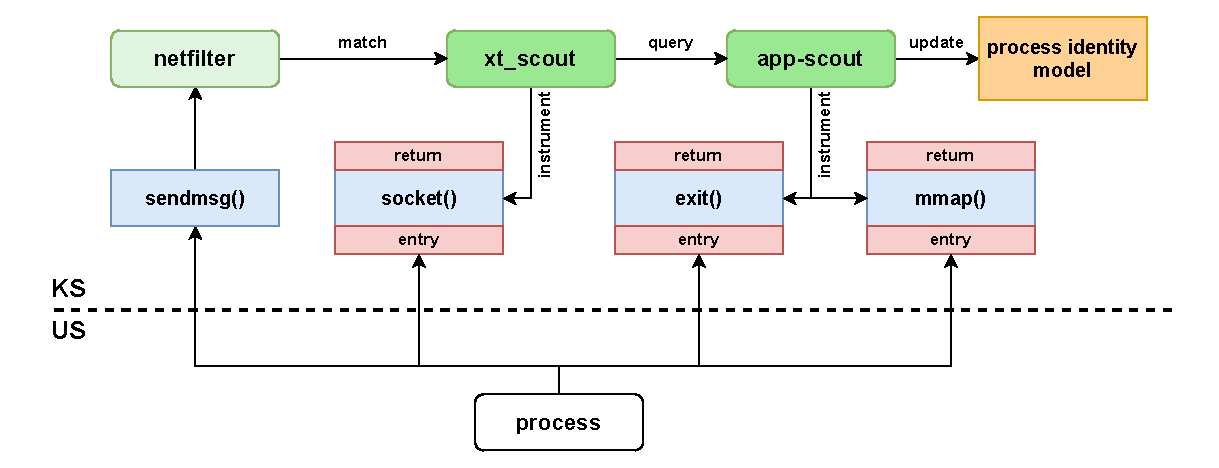
\includegraphics[width=\textwidth,keepaspectratio]{figures/appscout-architecture.pdf}
    \caption{\scout{} architecture for traffic filtering.}
    \label{appfw:appscout:fig:sys-architecture}

    \vspace{-32pt}
\end{figure}


\subsubsection{System overview}

\scout{} instruments certain kernel functions that are invoked during the life
cycle of a process. During its initial setup phase, the dynamic linker (i.e.,
\texttt{ld-linux}) maps the necessary shared objects into virtual memory, one
section at a time, with the appropriate permissions (e.g., r-x for
\textit{.text}, rw- for \textit{.data}, etc.) These, along with any other
objects that may be dynamically loaded on demand after control is ceded to the
base binary, are accounted for by this module and attributed to their respective
process. This information can either be relinquished after the termination of
said process, or persist until the module is unloaded. The former alternative is
preferable for memory-constrained systems, or when the identity of a process
becomes unnecessary after its termination (e.g., network traffic filtering).
The latter alternative is preferable when processor time is indispensable, or
when \scout{} is employed for auditing purposes.

\texttt{xt\_scout} is the kernel segment of an \texttt{iptables} extension that
we developed for matching packets based on the identity of their originating
process. Since \texttt{app-scout} is the only module with access to the process
identity model, it also implements the lookup mechanism for the identity of a
certain process. However, it is not immediately clear from the perspective of a
Netfilter match callback what that process should be. In newer kernel versions,
the socket no longer contains information regarding the process that created it.
While it still retains knowledge of user and group ownership in order not to
break compatibility with the \texttt{owner} extension in \texttt{iptables}, this
data is insufficient for our purposes. As a result, the \texttt{xt\_scout}
module instruments the creation of new sockets by userspace tasks and attributes
them a process ownership. This relation between a socket and its owner process
is then leveraged during the evaluation of an \texttt{iptables} rule to query
the \texttt{app-scout} module.


\subsubsection{Security considerations}

In order to facilitate the easy adoption of \scout{} we decided against
modifying the kernel source and instead implementing it as a collection of
loadable modules. A consequence of this decision is that the process state prior
to their insertion into the kernel cannot be accounted for. Thus, we recommend
that the \scout{} modules be included in the initial ramdisk of the system and
be loaded prior to the \texttt{init} process pivoting the root filesystem. In
this scenario, we consider the initramfs to be part of the Trusted Computing
Base (TCB) of the system.

In order to guarantee the authenticity and integrity of the modules, we suggest
employing the module signing facility of the kernel (based on X.509 ITU-T
standard certificates). In lieu of this option, the entire initial ramdisk
should be verified by its bootloader. E.g., on ARM systems that adhere to the
ARM Trusted Firmware Design and use U-Boot as BL33, the Firmware $\mu{}$Image
Package that contains the kernel and ramdisk can be signed by the developer and
verified at boot time. The public key used in the signature verification can
either be hardcoded in the U-Boot binary or loaded from its Flattened Device
Tree, both being themselves verified by the Original Equipment Manufacturer
(OEM) bootloader.

In our threat model, we consider the attacker capable of gaining access to the
system but require that the \scout{} modules had already been loaded at that
time. If the attacker is considered to be able of escalating his privilege level
to that of \textit{root}, we require that the kernel be put in lockdown via
\textit{securityfs} immediately after loading the \scout{} modules. Otherwise,
the attacker can either reload the \texttt{app-scout} module or interfere with
it via a module of his own, with the purpose of obfuscating his intrusion
attempt during auditing or staging further attacks.

%%%%%%%%%%%%%%%%%%%%%%%%%%%%%%%%%%%%%%%%%%%%%%%%%%%%%%%%%%%%%%%%%%%%%%%%%%%%%%%%
\subsection{Implementation}
\label{apffw:appscout:implementation}

In this section we present implementation details for the \texttt{app-scout} and
\texttt{xt\_scout} kernel modules, motivating our choice for instrumentation and
discussing the benefits and limitations of a potential Linux Security Module
(LSM) alternative.


\subsubsection{An argument for instrumentation}

It was clear from the outset that in order to build a system-wide, long-term
process identity model, we needed to collect certain information at runtime.
This information is not always readily accessible (i.e., stored in kernel
structures, but instead transient - in the local context of a call frame) and
must be obtained and indexed before the process state change that it represents
propagates to userspace. For example, if a process maps a file in its virtual
address space, our solution must intercept this operation and analyze the
contents of the mapped file before said process has a chance to acknowledge that
the operation finalized successfully and potentially modify the memory, or unmap
it.

There are two approaches to this problem: either manually adding hooks in
certain key functions, or instrumentation. While the former is a valid approach
(e.g., the integration method of the Netfilter system into the Linux kernel),
unless merged into upstream it will deter adoption of this system, primarily by
teams that develop their own Linux fork; a fairly common practice in the
embedded industry. Consequently, an instrumentation-oriented approach would be
preferable. This decision also presents us with another choice, between static
and dynamic instrumentation. Although the static approach (i.e., performed at
compile time) yields less overhead, the difficulty of its implementation coupled
with the reduced set of targets that need to be instrumented renders it
inefficient. Our view on this issue is further affirmed by past optimizations to
the kprobes system (i.e., the dynamic instrumentation framework of the kernel).

Initially, kprobes were computationally expensive due to the use of software
interrupts to trap the execution of certain kernel code regions. Incidentally,
this approach is also used by debuggers via the \texttt{ptrace()} system call.
However, debuggers are required to employ it due to their inferiors (i.e.,
programs under test) being separate processes. In 2010, a patchset by the author
of Djprobe \cite{hiramatsu2007djprobe} implemented the jump optimization for
kprobes, reducing their overhead to almost negligible margins. At the time of
writing, this optimization is available on x86, ARM and PowerPC. Taking into
consideration the fact that over ten years later, improvements are still being
researched \cite{jia2024fast}, we considered kprobes to be a viable choice for
runtime data collection via instrumentation.


\subsubsection{Construction of process identity}

The goal of the \texttt{app-scout} module is to gradually create a process
identity model based on data obtained from instrumentation. This model is
organized as an associative array using process IDs as keys for easy retrieval.
Ideally, the process identity information would have been stored in its
respective \texttt{task\_struct} instance. However, this structure has very few
fields that could be repurposed and doing so could very well interfere with
other mechanisms. E.g., the \texttt{security} field would be a prime candidate
if not for the fact that it is reserved for LSMs such as Tomoyo. Moreover, the
\texttt{task\_struct} instance is released after the termination of the process,
meaning that the reference to the process identity information would have been
lost at the time of a post-mortem audit.

The data associated to each PID in our model consists primarily of a list of
SHA256 digests computed based on the contents of each executable memory-mapped
region. Writable data sections have been excluded based on their volatile
nature. While an argument could be made in favor of including \textit{.rodata}
sections in our model, we consider that the \textit{.text} sections are
sufficient for demonstrating the capabilities of this prototype. Furthermore, we
acknowledge the possibility of encountering writable, non-file-backed executable
sections in processes that implement JIT compilers or translators. Efficiently
labeling a continuously mutating memory region at any given time is in and of
itself a non-trivial task, let alone tracking its change history during the
runtime of the process. Other solutions such as \texttt{Dymo}
\cite{gilbert2011dymo} reason that code generated by a trusted binary should
itself be trusted. Based on these considerations, we decided to take a similar
stance and deem the identification of JIT-ed code outside the scope of this
paper.

In order to retrieve the aforementioned data, we initially wanted to instrument
\texttt{do\_mmap()} due to it being a common path for the \texttt{mmap()} system
call but also for Asynchronous I/O (AIO) and Inter-Process Communication (IPC)
mechanisms. However, this function is called while holding the virtual memory
area lock for the current process. Normally, this would not be an issue.
However, our instrumentation callback performs one particularly costly operation
that can force the current task to yield. As a result, we selected
\texttt{vm\_mmap\_pgoff()} (i.e., the caller of \texttt{do\_mmap()} on the
\texttt{mmap()} syscall path) instead.

In the pre-call probe, we exclude kernel threads from our analysis and ensure
that the region is supposed to be mapped with execute permissions. In the
post-call probe, we determine the virtual address where a known number of pages
have been mapped. Having obtained this address does not necessarily mean that
the actual data resides in memory. Consequently, we pin those pages in memory,
forcing the kernel to fault them into RAM if any are missing. Herein lies the
previously mentioned problem: depending on the underlying filesystem driver of
backing storage device driver, this operation can force the current task to
yield its remaining CPU time. We have first observed this behaviour in our
development environment, using the Plan 9 filesystem protocol. Because the
kprobe instrumentation callbacks are invoked in atomic context, we were required
to re-enable preemption for the duration of this operation. We reasoned that as
opposed to classical kprobes (i.e., those that are based on software
interrupts), the jump-optimized version that we use should be able to safely
execute even outside an atomic context. As a precautionary measure, we
arbitrarily increased the maximum number of concurrently active kprobe instances
for this function. After all pages are guaranteed to be present in main memory,
we calculate the SHA256 sum and store it alongside the name of the backing file
in our data structure. Finally, the memory pin is released in order to prevent
an unsustainable growth of the Resident Set Size (RSS).

In order to prevent the unbounded growth of kernel memory usage for the process
identity model data structures, we have implemented a garbage collection
mechanism. By instrumenting \texttt{do\_exit()}, we intercept the termination of
a process and schedule a delayed deletion of its information. The reason why we
do not perform this action immediately is that other modules may still process
related events. For example, packets emitted by said process could still be
traversing the network stack after its death. Consequently, the
\texttt{xt\_scout} module may query \texttt{app-scout} regarding its identity in
order to reach a match verdict.


\subsubsection{Xtables integration}

The \texttt{iptables} extension consists of two components. One is the shared
object \texttt{libxt\_scout.so} that implements the necessary functionality for
the userspace tool (e.g., argument parsing, rule printing, etc.)
\texttt{iptables} loads this plugin on demand from certain well known paths
(e.g., \texttt{/usr/lib/xtables}) or from the paths stored in the
\texttt{XTABLES\_LIBDIR} environment variable.

The second component is the \texttt{xt\_scout} kernel module. This module
implements the \texttt{checkentry()} and \texttt{match()} callbacks for the
Xtables framework. The former performs sanity checks on newly inserted rules.
The latter is invoked as part of a potentially larger rule evaluation on a
specific packet or rather, a \texttt{sk\_buff} object. In Section
\ref{apffw:appscout:architecture} we mentioned that this socket buffer instance can be
linked back to the socket that it belongs to. However, that socket is not itself
linked to any given process in newer kernel versions. Nonetheless, there is a
mechanism in place for this.

A process can be assigned as the owner of socket in order for the kernel to send
signals under certain conditions. One of the more relevant examples is being
notified when urgent data is available as part of a TCP stream. Nonetheless,
even Urgent Pointers are largely unsupported in modern applications, many TCP/IP
network stacks preferring to handle urgent data in the same queue as normal data
instead of implementing a fast path. As a result, the \texttt{xt\_scout} module
instruments the \texttt{soc\_alloc\_file()} function. This function is invoked
after the successful instantiation of a socket in order to allocate a
\texttt{file} structure and bind the socket to a file descriptor. In our
instrumentation callback, we initialize the ownership field with the PID of the
current process (i.e., the one that created the socket). Thus, we create a
persistent link between a socket object and a process entry in our
\texttt{app-scout} model.

\begin{lstlisting}[
    style=bashstyle,
    caption={iptables rule with scout and conntrack modules},
    label={apffw:appscout:lst:rule}
]
$ iptables                                             \
    -m conntrack -m scout `# load extension modules  ` \
    -I OUTPUT             `# insert on OUTPUT chain  ` \
    -j DROP               `# DROP verdict on match   ` \
    --digest  9986...7ae7 `# SHA256 digest (abridged)` \
    --ctstate NEW         `# new connection          `
\end{lstlisting}


The benefit of integrating \texttt{app-scout} with the \texttt{Xtables}
framework is that all other \texttt{iptables} extensions are readily available
to the user. For example, Listing \ref{apffw:appscout:lst:rule} illustrates a
rule that makes use of the \texttt{conntrack} module to block the creation of a
new connection based on application identity. Without it, the match callback
function in \texttt{xt\_scout} would be invoked for every single outgoing
packet, even though the verdict is predictable and should be memoized. Note
however that the order in which the modules are loaded is more important than
the order in which the match criteria is specified. The only reason why the
\texttt{scout} module is not invoked on subsequent packets is that the
\texttt{ctstate} check failed beforehand. If the command line invocation were to
be changed (on the second line) such that the \texttt{scout} module would be
specified first, then the \texttt{Xtables} framework would always invoke the
process identity match function, thus negating the advantage of using
\texttt{conntrack}.


\subsubsection{Incompatibility between kprobes and LSMs}
\label{appfw:appscout:incompatibility}

In an early prototype, we considered implementing \scout{} as a LSM in order to
provide a guarantee with regard to its initialization order in the Linux kernel
boot sequence. Because we did not intend for it to be yet another Mandatory
Access Control (MAC) extension but instead only a monitoring mechanism, we
avoided introducing new security hooks in the kernel.

When attempting to instrument the \texttt{vm\_mmap\_pgoff()} function with
jump-optimized kretprobes, we noticed a critical flaw. The new kprobe system
creates an instruction cache buffer for storing whatever is replaced with an
\texttt{int 3} or \texttt{jmp} instruction during instrumentation. These buffers
are allocated in page-sized units. In order to determine how many instructions
could be cached in one page, the 4KB page size is divided by the maximum
instruction size for the current architecture. While it is known that this value
is 15 for x86-64, the associated variable remains uninitialized until
\texttt{init\_kprobes()} is executed at runtime. Since LSM initializer functions
are invoked earlier than those of other modules (or even core components),
trying to register a jump optimized kprobe will lead to a kernel panic caused
by a division-by-zero exception.

%%%%%%%%%%%%%%%%%%%%%%%%%%%%%%%%%%%%%%%%%%%%%%%%%%%%%%%%%%%%%%%%%%%%%%%%%%%%%%%%
\subsection{Evaluation}
\label{apffw:appscout:evaluation}


\subsubsection{Experimental setup}

The experiments described in this section have been carried out on the following hardware:

\begin{itemize}
    \item \textbf{Intel NUC:} Intel Core i7-7567U CPU @3.50GHz, Intel I219-V 1-Gigabit Ethernet Controller, 8GB DDR4 memory @2400MT/s.
    \item \textbf{IBM System x3550 M4:} Intel Xeon E5-2650Lv2 CPU @1.70GHz, Intel 82599ES 10-Gigabit SFP+ Ethernet Controller, 32GB DDR3 memory @1600MT/s.
\end{itemize}

The reported throughput was derived from the \texttt{iperf3} output and was based on the application data transfer, excluding any headers. Both systems are running a minimal installation of Arch Linux with kernel version 6.11.0.

\subsubsection{Throughput impact}

%% metodology
Our throughput evaluation of \scout{} consists of \texttt{iperf3} tests performed between directly linked systems. For each testing campaign we have varied the Maximum Transmission Unit (MTU) between 100 and the maximum value supported by the NIC. For each \texttt{iperf3} experiment, we have used the reported average data transfer rate over a TCP connection lasting ten seconds. The reported values do not include the header lengths of the underlying network layers.

\begin{figure*}
    \centering

    \begin{tikzpicture}
        \begin{axis}[
            restrict y to domain = 9420:9440,
            width                = \textwidth,
            height               = 5cm,
            at                   = {(0,0)},
            xmin                 = 1000,
            xmax                 = 9400,
            ymin                 = 9431.5,
            ymax                 = 9436.5,
            xtick distance       = 1000,
            ytick distance       = 1,
            grid                 = both,
            xlabel               = {MTU [bytes]},
            ylabel               = {Throughput [Mbps]},
            legend columns       = 3,
            legend style         = {at={(0.17,1.05)}, anchor=south west}
        ]
            \addplot[color=Blue, very thick]
                table[x=mtu, y=baseline, col sep=comma]
                {src/chapters/04-AppIdFirewall/data/cocos-throughput-ma30.csv};
            \addlegendentry{baseline}

            \addplot[color=Red, very thick]
                table[x=mtu, y=scout, col sep=comma]
                {src/chapters/04-AppIdFirewall/data/cocos-throughput-ma30.csv};
            \addlegendentry{AppScout}

            % function derived based on scipy.stats.linregress
            \draw[Green, dashed, line width=1.5pt] plot[samples=2, domain=1000:9420]
                function {0.000102 * x + 9432.945001};
            \addlegendimage{Green, dashed, line width=1.5}
            \addlegendentry{lin. regression}
        \end{axis}
    \end{tikzpicture}

    \caption{\scout{} throughout on IBM system.}
    \label{apffw:appscout:fig:cocos-throughput}
\end{figure*}

\radu{TODO: check why the draw command does not work here}


Figure \ref{apffw:appscout:fig:cocos-throughput} consists of three campaigns of tests, illustrating the impact of adding one \texttt{iptables} rule consisting of strictly one \texttt{xt\_scout} match function invocation. The match argument was selected so that each query to \texttt{app-scout} would parse the executable sections record in its entirety, thus simulating a worse case scenario. For \texttt{iperf3}, this record consists of 13 entries. Because the average throughput difference between the baseline and the filtered case is exceedingly low (0.15 Mbps) within the MTU range 1500-9710, we performed a moving average with a window of 30 samples, equating to 300 bytes. This was necessary in order to demonstrate that the low overhead was not coincidental. Moreover, we observe a tendency of the \scout{} throughput to grow and converge towards the baseline for increasingly higher MTU values (see the linear regression of the raw data in the 1500-9710 MTU range). This phenomenon can be motivated by a decrease in the number of Packets Per Second (PPS). For example, a six-fold increase over the default MTU size of 1500 translates results in a similar decrease in the number of packets necessary to saturate the network controller. Because the process identity inference cost does not depend on the packet size, it stands to reason that the \scout{} overhead should also decrease sixfold.

\begin{figure*}[h]
    \centering

    \begin{tikzpicture}
        \begin{axis}[
            restrict y to domain = 953:957,
            width                = \textwidth,
            height               = 5.2cm,
            at                   = {(0,0)},
            xmin                 = 1000,
            xmax                 = 8700,
            ymin                 = 954.5,
            ymax                 = 957.0,
            xtick distance       = 1000,
            ytick distance       = 0.5,
            x tick label style   = {rotate=45},
            grid                 = both,
            xlabel               = {MTU [bytes]},
            ylabel               = {Throughput [Mbps]},
            legend columns       = 3,
            legend style         = {at={(0.03,0.78)}, anchor=south west}
        ]
            \addplot[color=Blue, very thick]
                table[x=mtu, y=baseline, col sep=comma]
                {src/chapters/04-AppIdFirewall/data/nuc-throughput-ma30.csv};
            \addlegendentry{baseline}

            \addplot[color=Red, very thick]
                table[x=mtu, y=scout, col sep=comma]
                {src/chapters/04-AppIdFirewall/data/nuc-throughput-ma30.csv};
            \addlegendentry{AppScout}
        \end{axis}
    \end{tikzpicture}

    \caption{\scout{} throughout on Intel NUC.}
    \label{apffw:appscout:fig:nuc-throughput}
\end{figure*}


Similarly, Figure \ref{apffw:appscout:fig:nuc-throughput} illustrates the same experiment performed on the Intel NUC system, with a 1Gbps NIC. Although less noisy due to the lower throughput, the same moving average window was used for consistency. Despite a number of anomalies that can for the most part be attributed to the \texttt{e1000e} driver, we notice that the reduced number of Packets Per Second (PPS) in relation to the core count as well as the increase base CPU frequency contribute to further reduce the overhead of \texttt{xt\_scout}.


\subsubsection{System tuning based on processor resources}
\label{subsec:tuning}

During our experiments, we encountered an issue where \scout{} caused the network device watchdog timer to trigger, leading to cascading resets of the NIC. Normally, this problem is caused by faulty hardware that is unable to service the transmission queue in a reasonably timely manner. However, this bug can also be triggered on Intel network controllers by setting a high value for the \texttt{InterruptThrottleRate} driver argument. This commandline kernel argument is used to limit the number of interrupts generated by the NIC in situations where most of the CPU time is dedicated to network traffic processing. In our case, the process identity lookup operation introduced a delay that had the same effect as the throttle mechanism. We identified three solutions to this problem:

\begin{enumerate}
    \item \textbf{Adjust the frequency governor:} When we first triggered this bug, the effective CPU frequency was set to approx. 1.1GHz. By setting the scaling governor to \textit{performance} mode, we increased it to a mostly constant 2.1GHz, thus compensating for the identity lookup delay.

    \item \textbf{Disable garbage collection:} Avoiding scheduling more delayed work in the bottom half is a good method of freeing up clock cycles. While still using the default \textit{userspace} scaling governor, we noticed an approx. 80\% decrease in watchdog timer triggers. While this was not a permanent solution in our testing environment, it can have a greater impact on servers with high system load and many short-lived processes.

    \item \textbf{Employ conntrack:} The \texttt{conntrack} module can be used to improve the efficiency of \texttt{iptables} by reducing the number of match callback invocations based on the state of each connection. This type of optimization is widely used in both hardware and software firewalls and can have a greater impact than any of the previous solutions.
\end{enumerate}

\subsubsection{Identity auditing using the Netlink protocol}

Traditionally, arbitrary communication between a userspace process and a specific kernel module was done via the Virtual File System (VFS) layer. Lately, this functionality has been partially duplicated via Netlink sockets, with specific modules exposing different subsystems as protocols in the \texttt{AF\_NETLINK} domain. For example, \texttt{netstat} is superseded by \texttt{ss} which uses the Netlink Socket Diagnostics subsystem. Similarly, \texttt{nftables} uses the Netlink Netfilter subsystem which was backported to the \texttt{iptables} backend to maintain compatibility.

As a result, we decided to implement support for a new Netlink subsystem in the \texttt{app-scout} module. We offer \texttt{probe\_appscout} as a userspace application capable of querying the kernel module for information regarding a certain process, based on its PID. Listing \ref{lst:audit} illustrates its use and how the \texttt{app-scout} module can account for dynamically loaded objects that are not included as dependencies in the ELF file. In this example, using \texttt{ls} with the long listing format flag triggers the on-demand loading of the \texttt{gcc} runtime library and mathematical library (for file size calculations), as well as the \texttt{systemd} Name Service Switch library (for user or group name lookup by ID).

\begin{lstlisting}[
    style=bashstyle,
    caption={Userspace interaction with \scout{} LKM},label={lst:audit}
]
$ ldd $(which ls)
    linux-vdso.so.1
    libcap.so.2 => /usr/lib/libcap.so.2
    libc.so.6 => /usr/lib/libc.so.6
    ld-linux-x86-64.so.2 => /usr/lib64/ld-linux-x86-64.so.2

$ probe_appscout 209        # comm = "ls"
    caf8....4ebb -- libc.so.6
    fbc2....c4c5 -- libcap.so.2.70
    ce73....71ec -- ld-linux-x86-64.so.2
    82ae....2896 -- ls

$ probe_appscout 210        # comm = "ls -l"
    b2f3....9eb1 -- libgcc_s.so.1
    e5e2....6cd0 -- libm.so.6
    5854....999c -- libnss_systemd.so.2
    <remaining output is identical to PID=209>
\end{lstlisting}

We note that one downside of using the Netlink framework is that dynamic allocation of protocol numbers is not currently supported. The well-established subsystems are assigned a static and contiguous block of numbers starting from zero that grows with each new upstreamed feature. At the moment, the Netlink framework has an arbitrary limit of 32 Netlink protocol numbers, of which 23 are reserved. Consequently, there is a chance of protocol number collision between the \texttt{app-scout} module and other drivers. The probability for this is higher on embedded devices that make use of third party drivers, especially considering that Netlink sockets can be used to disseminate sensor measurements to userspace.
